\documentclass[main.tex]{subfiles}
\begin{document}
\chapter{Quantum chromodynamics in practice}
\label{chapter:qcd}
    In the previous chapter we introduced the basic concepts
    of QCD and setup the framework of calculating
    cross-sections. Cross-sections are the most relevant
    quantities to compute as they can be measured
    experimentally, and are a property of the particles
    being collided, rather than depending on the
    specifics of the experimental procedure.
    This provides a bridge to compare
    theoretical predictions and experiment.
    From (\ref{eqn:dsigma}, the partonic cross-section
    is the matrix element integrated over the relevant
    final-state phase-space, normalised by a flux factor.
    The matrix elements are
    calculated order-by-order in the strong coupling
    $\alpha_{s}$, (\ref{eqn:matrix_element}),
    where each order corresponds to a set of Feynman diagrams
    that have the appropriate number of vertices,
    as each QCD vertex brings along a factor of $\alpha_{s}$.

    In this chapter we will discuss the problems that
    arise when evaluating these Feynman diagrams and outline
    some solutions that have been widely adopted to circumvent
    these issues to provide real-world applicable predictions.
    This chapter forms the theoretical foundations on which
    the work of this thesis is built upon.

    We will consider the divergent nature of matrix
    elements and introduce the most widely used techniques
    to tame these singularities.

\section{Divergent structures}\label{sec:divergences}
    We have seen that matrix element computations
    result in evaluating Feynman diagrams. From
    the QCD Feynman rules (ref here), it becomes
    clear that integrating over all momentum modes
    will give rise to singularities. The divergences
    associated with high energy modes are ultraviolet
    (UV) divergences. On the opposite end of the energy
    spectrum, low energy modes also give rise to 
    infrared (IR) divergences.

    The de-facto methods to alleviate these
    divergences are through regularisation
    for UV divergences, and through subtraction
    schemes for IR divergences. Both of these
    methods will be discussed in this section.

\subsection{Ultraviolet divergences}\label{sec:UV}
    During intermediate steps of calculations,
    such as trying to compute loop diagrams,
    we have to evaluate integrals of the form
    \begin{equation}\label{eqn:loop_integral}
        \int_{0}^{\Lambda} \dfrac{\mathrm{d}^{4}\ell}{(2\pi)^{4}}\dfrac{1}{\ell^{2}(\ell+p)^{2}} \sim \log{\Lambda} \, ,
    \end{equation}
    where a cutoff scale $\Lambda$ has been introduced to
    capture the divergence as the loop momenta
    $k \rightarrow \infty$. It is clear that the
    integral diverges in this high energy limit,
    hence the name ultraviolet divergence.
    This UV divergence cannot influence the
    experimentally observable quantities at experiments,
    which are finite, because the final observable
    should not depend on the intermediate steps taken
    to get there.
    Infinities associated with UV divergences
    are removed via the process of renormalisation
    which introduces counterterms in the Lagrangian
    to exactly cancel these divergences.

    Before we introduce these counterterms, we
    first consider the procedure of regularisation
    which makes these infinities explicitly manifest.
    The most widely adopted method of regularisation
    is dimensional regularisation (DR) (cite here) which
    is based on the observation that the integral
    (\ref{eqn:loop_integral}), which is carried
    out in $d=4$ space-time dimensions, would be finite
    if $d < 4$.

    In DR we define $d = 4 - 2\epsilon$ such that
    after Feynman parametrisation (\ref{eqn:loop_integral})
    becomes
    \begin{equation}\label{eqn:dim_reg}
        \int \dfrac{\mathrm{d}^{d}\ell}{(2\pi)^{d}}\dfrac{1}{\ell^{2}(\ell+p)^{2}} = \dfrac{(-p^{2})^{-\epsilon}}{(4\pi)^{2-\epsilon}}\dfrac{\Gamma(1-\epsilon)^{2}}{\Gamma(2-2\epsilon)}\Gamma(\epsilon) \, ,
    \end{equation}
    where the divergence for $d = 4$, or equivalently
    $\epsilon \rightarrow 0$, is now captured in the
    Gamma function, $\Gamma(\epsilon)$. This becomes clear once
    we expand $\Gamma(\epsilon)$ around small $\epsilon$
    \begin{equation}\label{eqn:gamma_laurent}
        \Gamma(\epsilon) = \dfrac{1}{\epsilon} - \gamma_{E} + \dfrac{1}{2}\left(\gamma_{E}^{2} + \dfrac{\pi^{2}}{6}\right)\epsilon + \mathcal{O}(\epsilon^{2}) \, ,
    \end{equation}
    where $\gamma_{E} \approx 0.577$ is the Euler-Mascheroni
    constant, meaning the divergence is now regularised as a pole in
    $\epsilon$.

\subsection{Renormalisation}\label{sec:renormalisation}
    With the UV divergence regularised by dimensional
    regularisation, it is now possible to construct the forms
    of the counterterms order-by-order in $\alpha_{s}$ to
    explicitly cancel them.

    A subtlety with adjusting the dimension of the theory
    from $d=4$ to arbitrary dimensions is that the mass dimension
    of the Lagrangian has to change accordingly to retain a
    dimensionless action. We can account for this by
    introducing an arbitrary scale $\mu_{R}$, the renormalisation
    scale, into the gauge coupling
    constant to modify the mass dimension of the Lagrangian.
    For QCD this is done via the modification
    \begin{equation}\label{eqn:dimensionful_coupling}
        g_{s} \rightarrow g_{s}\mu_{R}^{\epsilon} \, .
    \end{equation}
    where it is understood the original gauge coupling is
    dimensionless. The order of $\mu_{R}$ is determined by examining
    the dimensions of the gauge and fermion fields
    in the Lagrangian (\ref{eqn:L_QCD}).
    We see that this introduces a scale dependence
    on the coupling constant $\alpha_{s}$, a point we will return
    to in \ref{sec:alpha_running}.
    % In a calculation,
    % intermediate steps will have a dependence on $\mu$,
    % however, once the $\epsilon \rightarrow 0$ limit
    % is taken the scale dependence drops out.

    The inclusion of counterterms into the theory can be
    thought of as renormalisations of the the bare fields
    and couplings in (\ref{eqn:L_QCD}) to restore predictive
    power to the theory. The renormalised fields and couplings
    can be given as (cite here)
    \begin{align}\label{eqn:renormlised_fields}
        \psi_{\mathrm{bare}} &= \sqrt{Z_{2}} \psi_{R} \, , \nonumber \\
        A_{\mathrm{bare}}^{\mu} &= \sqrt{Z_{3}} A_{R}^{\mu} \, ,\\
        g_{s,\mathrm{bare}} &= Z_{g} \mu_{R}^{\epsilon} g_{s,R} \, , \nonumber
    \end{align}
    where it conventional to define $Z_{1} = Z_{g}Z_{2}\sqrt{Z_{3}}$
    such that we can set $Z_{n} = 1 + \delta_{n}$ for $n \in \{1, 2, 3\}$.
    In this way we can write the Lagrangian as
    \begin{equation}
        \mathcal{L}_{\mathrm{renorm}} = \mathcal{L}_{\mathrm{bare}} + \mathcal{L}_{\mathrm{c.t.}} \, ,
    \end{equation}
    where the counterterms appearing in $\mathcal{L}_{\mathrm{c.t.}}$
    are determined by calculating $\delta_{n}$. There is freedom
    in the choice of $\delta_{n}$ which gives rise to
    different regularisation schemes. The minimal subtraction
    (MS) scheme subtracts only the epsilon pole appearing
    in loop integrals (\ref{eqn:gamma_laurent}). However, the most
    commonly used regularisation scheme is the modified minimal
    subtraction ($\overline{\mathrm{MS}}$) scheme which subtracts the
    epsilon pole plus a universal constant appearing in all
    loop integrals.

    In an all orders calculation of an observable,
    there would be no dependence on the renormalisation
    scale as it is a remnant of the regularisation prescription
    However, because in perturbative QCD observables
    are calculated order-by-order, there will be a residual
    dependence on the renormalisation scale stemming from
    the missing higher order terms. The conventional way
    that the community estimates the uncertainty associated
    with this residual dependence is by carrying out
    a scale variation. This involves evaluating the
    relevant quantities at the nominal renormalisation
    scale and again with the scale varied by a factor of
    two above and below.


\subsection{Running of the coupling constant}\label{sec:alpha_running}
    The bare coupling should not depend on the actual
    value of the renormalisation scale,
    \begin{equation}\label{eqn:d_g_bare_d_mu}
        \dfrac{\mathrm{d}g_{\mathrm{bare}}}{\mathrm{d}\mu_{R}} = 0 \, ,
    \end{equation}
    or said another way, the renormalisation process
    is independent of the renormalisation scale. The
    consequence of this is that $\alpha_{s}$ has to
    depends on the renormalisation scale.

    The behaviour of $\alpha_{s}$
    is governed by the Callan-Symanzik \cite{Callan:1970yg,Symanzik:1970rt}
    $\beta$-function
    \begin{equation}\label{eqn:beta_fn}
        \mu^{2} \dfrac{\partial \alpha_{s}(\mu^{2})}{\partial \mu^{2}} = \beta(\alpha_{s}) \, ,
    \end{equation}
    where the $\beta$-function can be written as a perturbative
    expansion in $\alpha_{s}$
    \begin{equation}\label{eqn:beta_series}
        -\beta(\alpha_{s}) = \alpha_{s}\sum_{n=0}^{\infty}\left(\dfrac{\alpha_{s}}{4\pi}\right)^{n+1} \beta_{n}\, 
    \end{equation}
    where the coefficients $\beta_{n}$ have been computed
    up to $\beta_{4}$ \cite{Baikov:2016tgj,Luthe:2017ttg}.
    The solution to (\ref{eqn:beta_fn}) to first order
    is
    \begin{equation}\label{eqn:1l_alpha}
        \alpha_{s}(\mu^{2}) = \dfrac{1}{\frac{\beta_{0}}{4\pi}\log\left(\frac{\mu^{2}}{\Lambda_{\mathrm{QCD}}^{2}}\right)} \, ,
    \end{equation}
    where $\Lambda_{\mathrm{QCD}}$ is the QCD scale,
    the scale at which $\alpha_{s}$ becomes
    large enough that perturbation theory breaks down,
    and $\beta_{0} = (11C_{A} - 4T_{R}n_{f})/3$.
    In QCD, $C_{A}=3$ and $T_{R}=\frac{1}{2}$, meaning for
    $n_{f} < \frac{33}{2}$ the sign of $\beta_{0}$ is positive,
    which is what we have observed in nature with six
    flavours of quarks. This behaviour of positive
    $\beta_{n}$ is also the case in all coefficients
    computed to date, meaning that $\alpha_{s}$
    decreases with increasing energy due to the minus sign
    in (\ref{eqn:beta_series}). This property is known as
    asymptotic freedom \cite{Gross:1973id,Politzer:1973fx},
    and is justification for treating QCD perturbatively.
    The running of the coupling constant has been
    observed experimentally as illustrated in Figure~\ref{fig:alpha_s_running}.
    \begin{figure}
        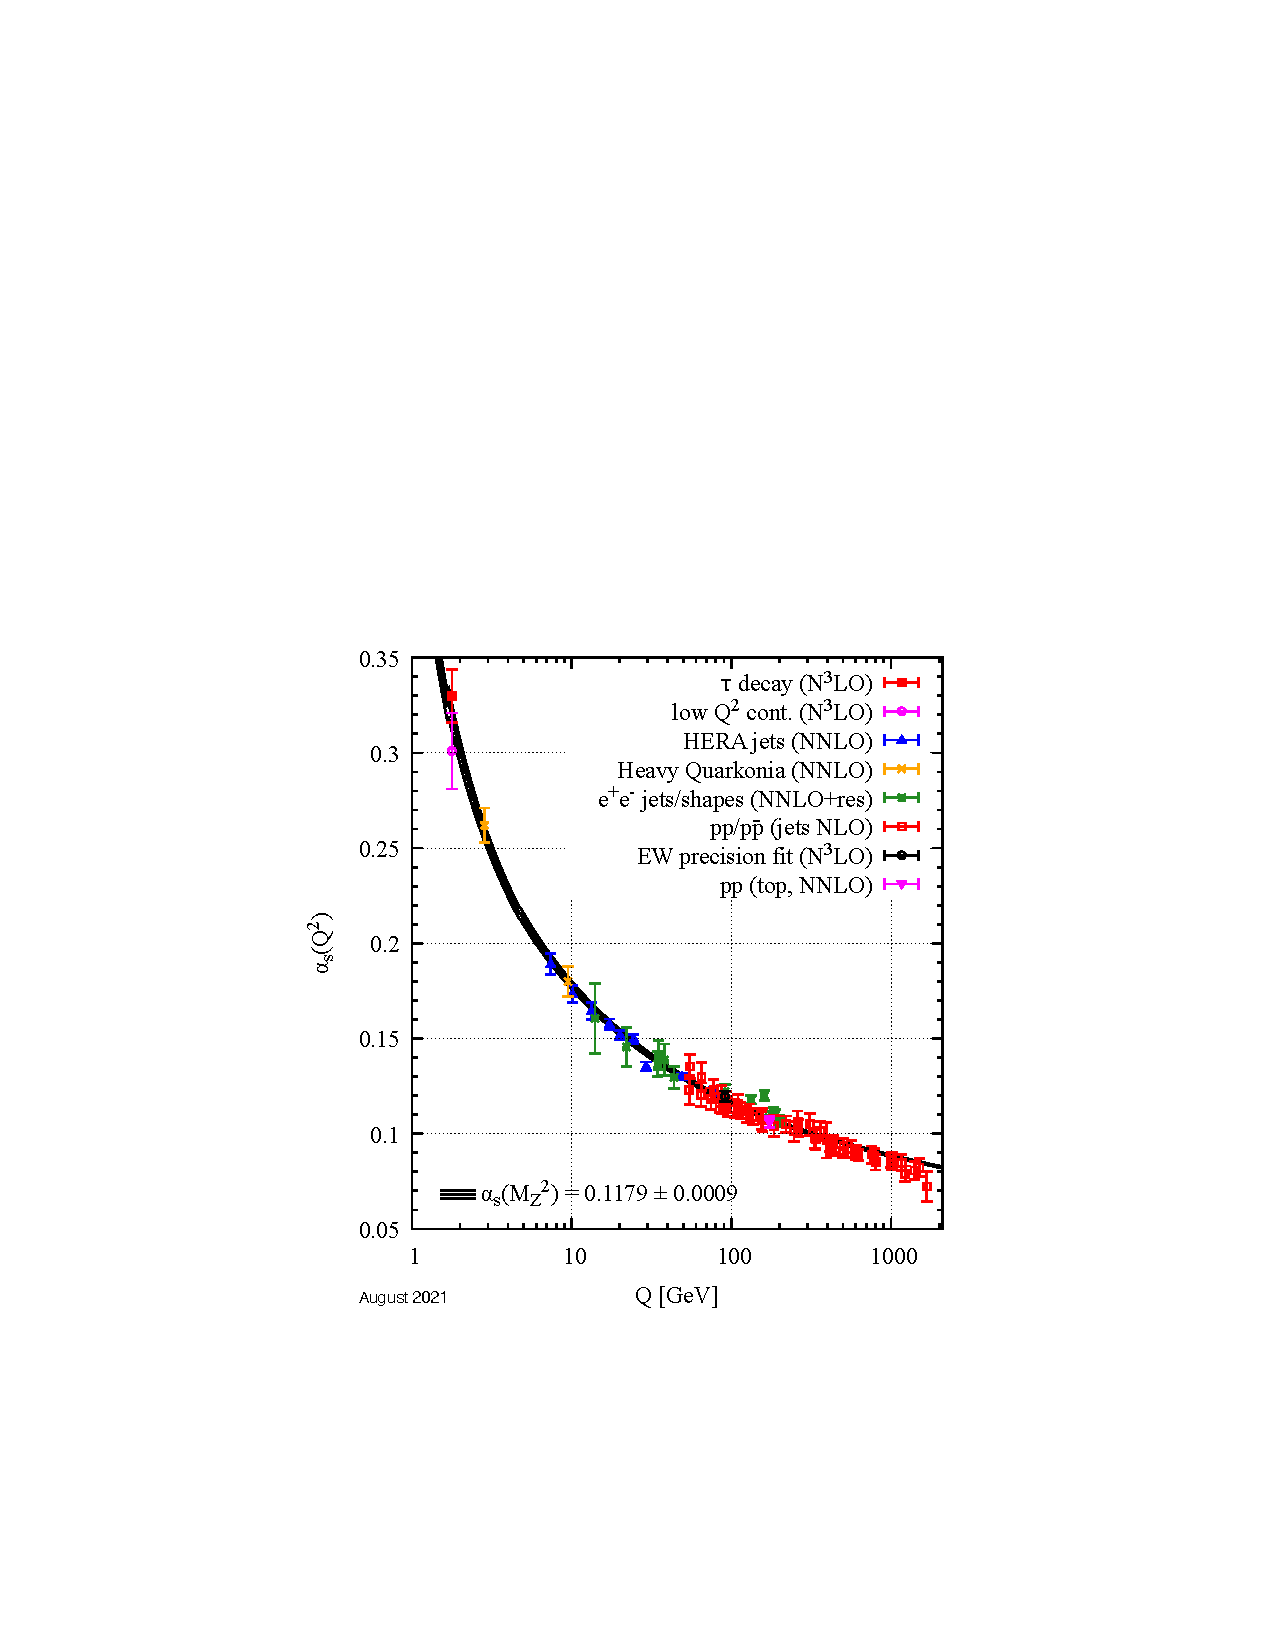
\includegraphics{qcd/alpha_s_running.pdf}
        \caption{The running of the strong coupling constant $\alpha_{s}$,
        as determined by experiments, with QCD theory prediction in black.
        Figure reference \cite{Workman:2022ynf}.}
        \label{fig:alpha_s_running}
    \end{figure}

    Another consequence of the running coupling
    is colour confinement, in which quarks and
    gluons cannot exist as free particles. Due
    to the increasing strength of coupling at low
    energies, quarks and gluons are forced to
    form composite, colourless particles. This means
    that at low energies, perturbative QCD
    is not an accurate description of nature,
    and the behaviour of hadrons cannot be predicted
    from perturbation theory.
\subsection{Infrared divergences}
    In Section~\ref{sec:UV} we saw how divergences
    stemming from high energy behaviour would occur
    in loop diagrams. On the other end of the energy
    spectrum we also have divergences from low energy
    modes. Since these divergences emerge from low energy
    behaviour they are called infrared (IR) divergences. There
    are two cases in which these divergences arise:
    in loop integrals (virtual) and when an emission
    of an extra particle (c.f. splitting functions
    \ref{eqn:AP_kernels}) has vanishing energy (soft),
    or becomes parallel to an external colourful line (collinear).

    Virtual IR divergences can be understood by looking
    at an integral of the form
    \begin{equation}\label{eqn:virtual_IR_integral}
        \int \dfrac{\mathrm{d}^{4}\ell}{(2\pi)^{4}} \dfrac{1}{\ell^{2}(\ell+p_{1})^{2}(\ell-p_{2})^{2}} \, ,
    \end{equation}
    which is encountered when calculating the one-loop
    virtual correction to the gluon-quark-antiquark vertex.
    It is clear that the denominator vanishes when $\ell \rightarrow 0$
    or when either $(\ell + p_{1})^{2}$ or $(\ell - p_{2})^{2} \rightarrow 0$.
    These situations correspond to the gluon in the loop propagator
    going soft, or collinear to the external quark or antiquark.
    These divergences are regulated in DR to give
    \begin{equation}\label{eqn:virtual_IR_DR}
    \end{equation}
    where we see a double $\epsilon$ pole corresponding to the
    soft and collinear divergence.

    Real IR divergences are manifest when integrating
    matrix elements over the phase-space of external state momenta.
    Matrix elements can be written as functions of Mandelstam variables
    \begin{equation}\label{eqn:mandelstam}
        s_{ij} = (p_{i} + p_{j})^{2} \xrightarrow[\mathrm{limit}]{\mathrm{massless}} 2 E_{i}E_{j}(1-\cos \theta_{ij}) \, ,
    \end{equation}
    where $p_{i}$ and $p_{j}$ are the 4-momenta of partons $i$ and $j$
    in the hard scattering.
    When either of the partons beecome soft, $E_{i,j}\rightarrow 0$,
    or when they go collinear to each other, $\theta_{ij} \rightarrow 0$,
    the matrix element will diverge if $s_{ij}$ appears
    in the demoninator. These scenarios correspond to an external
    particle becoming unresolved.

    In Section~\ref{sec:renormalisation}, we removed UV divergences
    through the use of counterterms to renormalise the theory, making
    predictions from the theory physical.
    IR divergences, on the other hand, arise even after the theory
    has been renormalised. The resolution to IR divergences is given by the
    Kinoshita-Lee-Nauenberg (KLN) theorem (cite here) which states
    that at each order of perturbation theory, the virtual and real
    contributions exactly cancel out, leaving only finite corrections.
    This cancellation occurs because the infrared pole structure is
    identical in the real and virtual corrections, but with an opposite sign.

    At a detector of a collider experiment, there is a finite
    energy resolution of the calorimeter. This means that
    it is not physically possible to observe arbitrarily soft
    partons. It is also not possible to distinguish two partons
    at arbitrarily small angles from one parton with the combined
    momenta. These limitations along with the KLN theorem
    means that any physical observable that we wish to predict
    with fixed-order perturbation theory must be insensitive to the
    emissions of soft or collinear partons. Any observable obeying
    this criteria is an infrared and collinear (IRC) safe observable.
    This leads to the concept of jets (cite here) which are collimated
    particles combined according to some jet algorithm.    

    In DR, the singularities from soft and collinear divergences
    are manifest as $\epsilon$ poles which makes the cancellation
    simple between the real and virtual parts. However, in practice, 
    the phase-space integrals of the matrix elements are rarely carried
    out analytically due to the high dimensionality of the integral.
    Instead they are done numerically with the use
    of Monte Carlo methods, which requires the integral to be in
    integer dimensions. Therefore, numerical techniques
    have been developed to deal with these IR divergences as well. The
    most common technique, subtraction, will be discussed in
    more detail in Section~\ref{sec:subtraction}.
    
\section{Factorisation of matrix elements}\label{sec:me_factorisation}
    In the previous section we examined the IR divergences
    that can arise in matrix elements, either explicitly
    through loop diagrams, or implicitly when carrying
    out the phase-space integral over the external state
    momenta. In this section we will discuss how these IR
    singularities are universal and can be factorised out
    of the matrix element. This property is exploited
    extensively in Sections ... where the research of this
    thesis is presented.

    

\subsection{Soft limits}\label{sec:me_soft}
\subsection{Collinear limits}\label{sec:me_collinear}

\section{Subtraction}\label{sec:subtraction}
\subsection{Catani-Seymour dipoles}\label{sec:CS_dipoles}
\subsection{Antenna}\label{sec:antenna_functions}
\end{document}